\documentclass{standalone}
\usepackage{pgfplots}
\pgfplotsset{compat=1.17}
\usetikzlibrary{arrows}
\tikzset{>=latex'}
\begin{document}
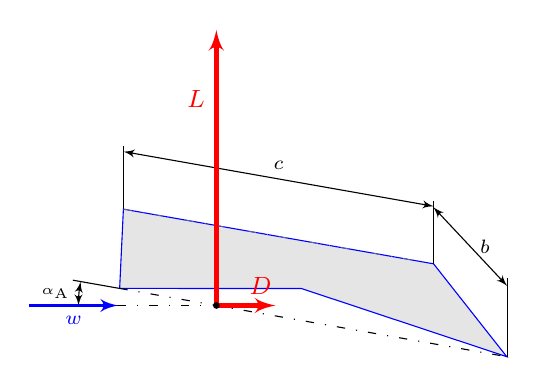
\begin{tikzpicture}[scale=5]

\begin{scope}[rotate around={-10:(.25,0)}] % Begin rotate

\begin{scope}[yshift=.2cm, xshift=-0.025cm,scale=.8] % Begin shift
    \filldraw[draw=blue,fill=gray!50!white,fill opacity=.4] (1.28,-.25) -- (1,0) -- plot file{naca643618_upper_half.dat} -- (0,0) -- (0.032,-.25) -- (0.6,-0.15) -- cycle;
    \draw[dotted, gray] plot file{naca643618_lower_half.dat};
    \draw[rotate around={10:(0,0)}] (0,0) -- (0,0.2);
    \draw[rotate around={10:(1,0)}] (1,0) -- (1,0.2);
    \draw[<->,xshift=-0.18] (-0.025,0.18) -- (0.975,0.18) node[above, midway]{\scriptsize{$c$}};
    \draw[loosely dash dot, gray,very thin] (0,0) -- (1,0);
    %\filldraw[gray] (0.25,0) circle (.2pt);
\end{scope} % End shift

\filldraw[draw=blue,fill=blue!30!white] plot file{naca643618.dat} -- cycle;
\draw[loosely dash dot] (0,0) -- (1,0);
\draw[rotate around={10:(1,0)}] (1,0) -- (1,0.2);
\draw[<->,rotate around={10:(1,0)}] (1,0.18) -- (.8125,.38) node[right,midway]{\scriptsize{$b$}};
%\draw[dash dot,gray] (0.25,0) -- (0.175,.2);
\draw (0,0) -- (-.12,0);

\begin{scope}[line cap=round,red,ultra thick, rotate around={10:(.25,0)}] % Lift and Drag Forces
    \draw[->] (.25,0) -- (.25,.7) node[near end,left]{\small{$L$}};
    \draw[->] (.25,0) -- (.4,0) node[near end,above]{\small{$D$}};
\end{scope}

\end{scope} % End rotate

\filldraw (.25,0) circle (.2pt);
\draw[loosely dash dot] (0,0) -- (.25,0);
\draw (0,0) -- (-.12,0);
\draw[<->] (-.1,0) arc (180:170:.35) node[midway,left]{\tiny{$\alpha_\textnormal{A}$}};
\draw[blue,->,very thick] (-.225,0) -- (0,0) node[below,midway]{\scriptsize{$w$}};
\end{tikzpicture}
\end{document}